\section{Design}
\label{sec:methodology}
% \wajih{Do a GLOBAL SEARCH of the paper and replace federated graph learning with federated provenance graph learning and replace anomaly detection with GNN-based anomaly detection where ever appropriate}


\subsection{Problem Formulation \& Overview}

Let \( C = \{Client_1, Client_2, \ldots, Client_k\} \) denote the set of client machines, where each machine \( Client_i \), for \( i = 1, 2, \ldots, k \), locally maintains its \logs to preserve privacy, ensuring that raw logs do not leave the machine. Our objective is to detect anomalous nodes within the client's provenance graphs, \( \{G_{c_1}, G_{c_2}, \ldots, G_{c_P}\} \), generated from these logs. To this end, we propose training a set of global \gnnshort models to model the benign behavior exhibited across all client logs without centralizing the log data.

Additionally, we aim to develop a global semantic encoder, \( \mathcal{E}_{\text{semantic}} \), capable of converting contextual attributes into vector space, thereby generating feature vectors for training our GNN models. Using these global \gnnshort models, we aim to identify anomalous nodes in provenance graphs constructed from \logs during runtime. These anomalies could be potential threats as their system activity significantly differs from benign patterns.



\begin{figure*}[t!]
  \centering
  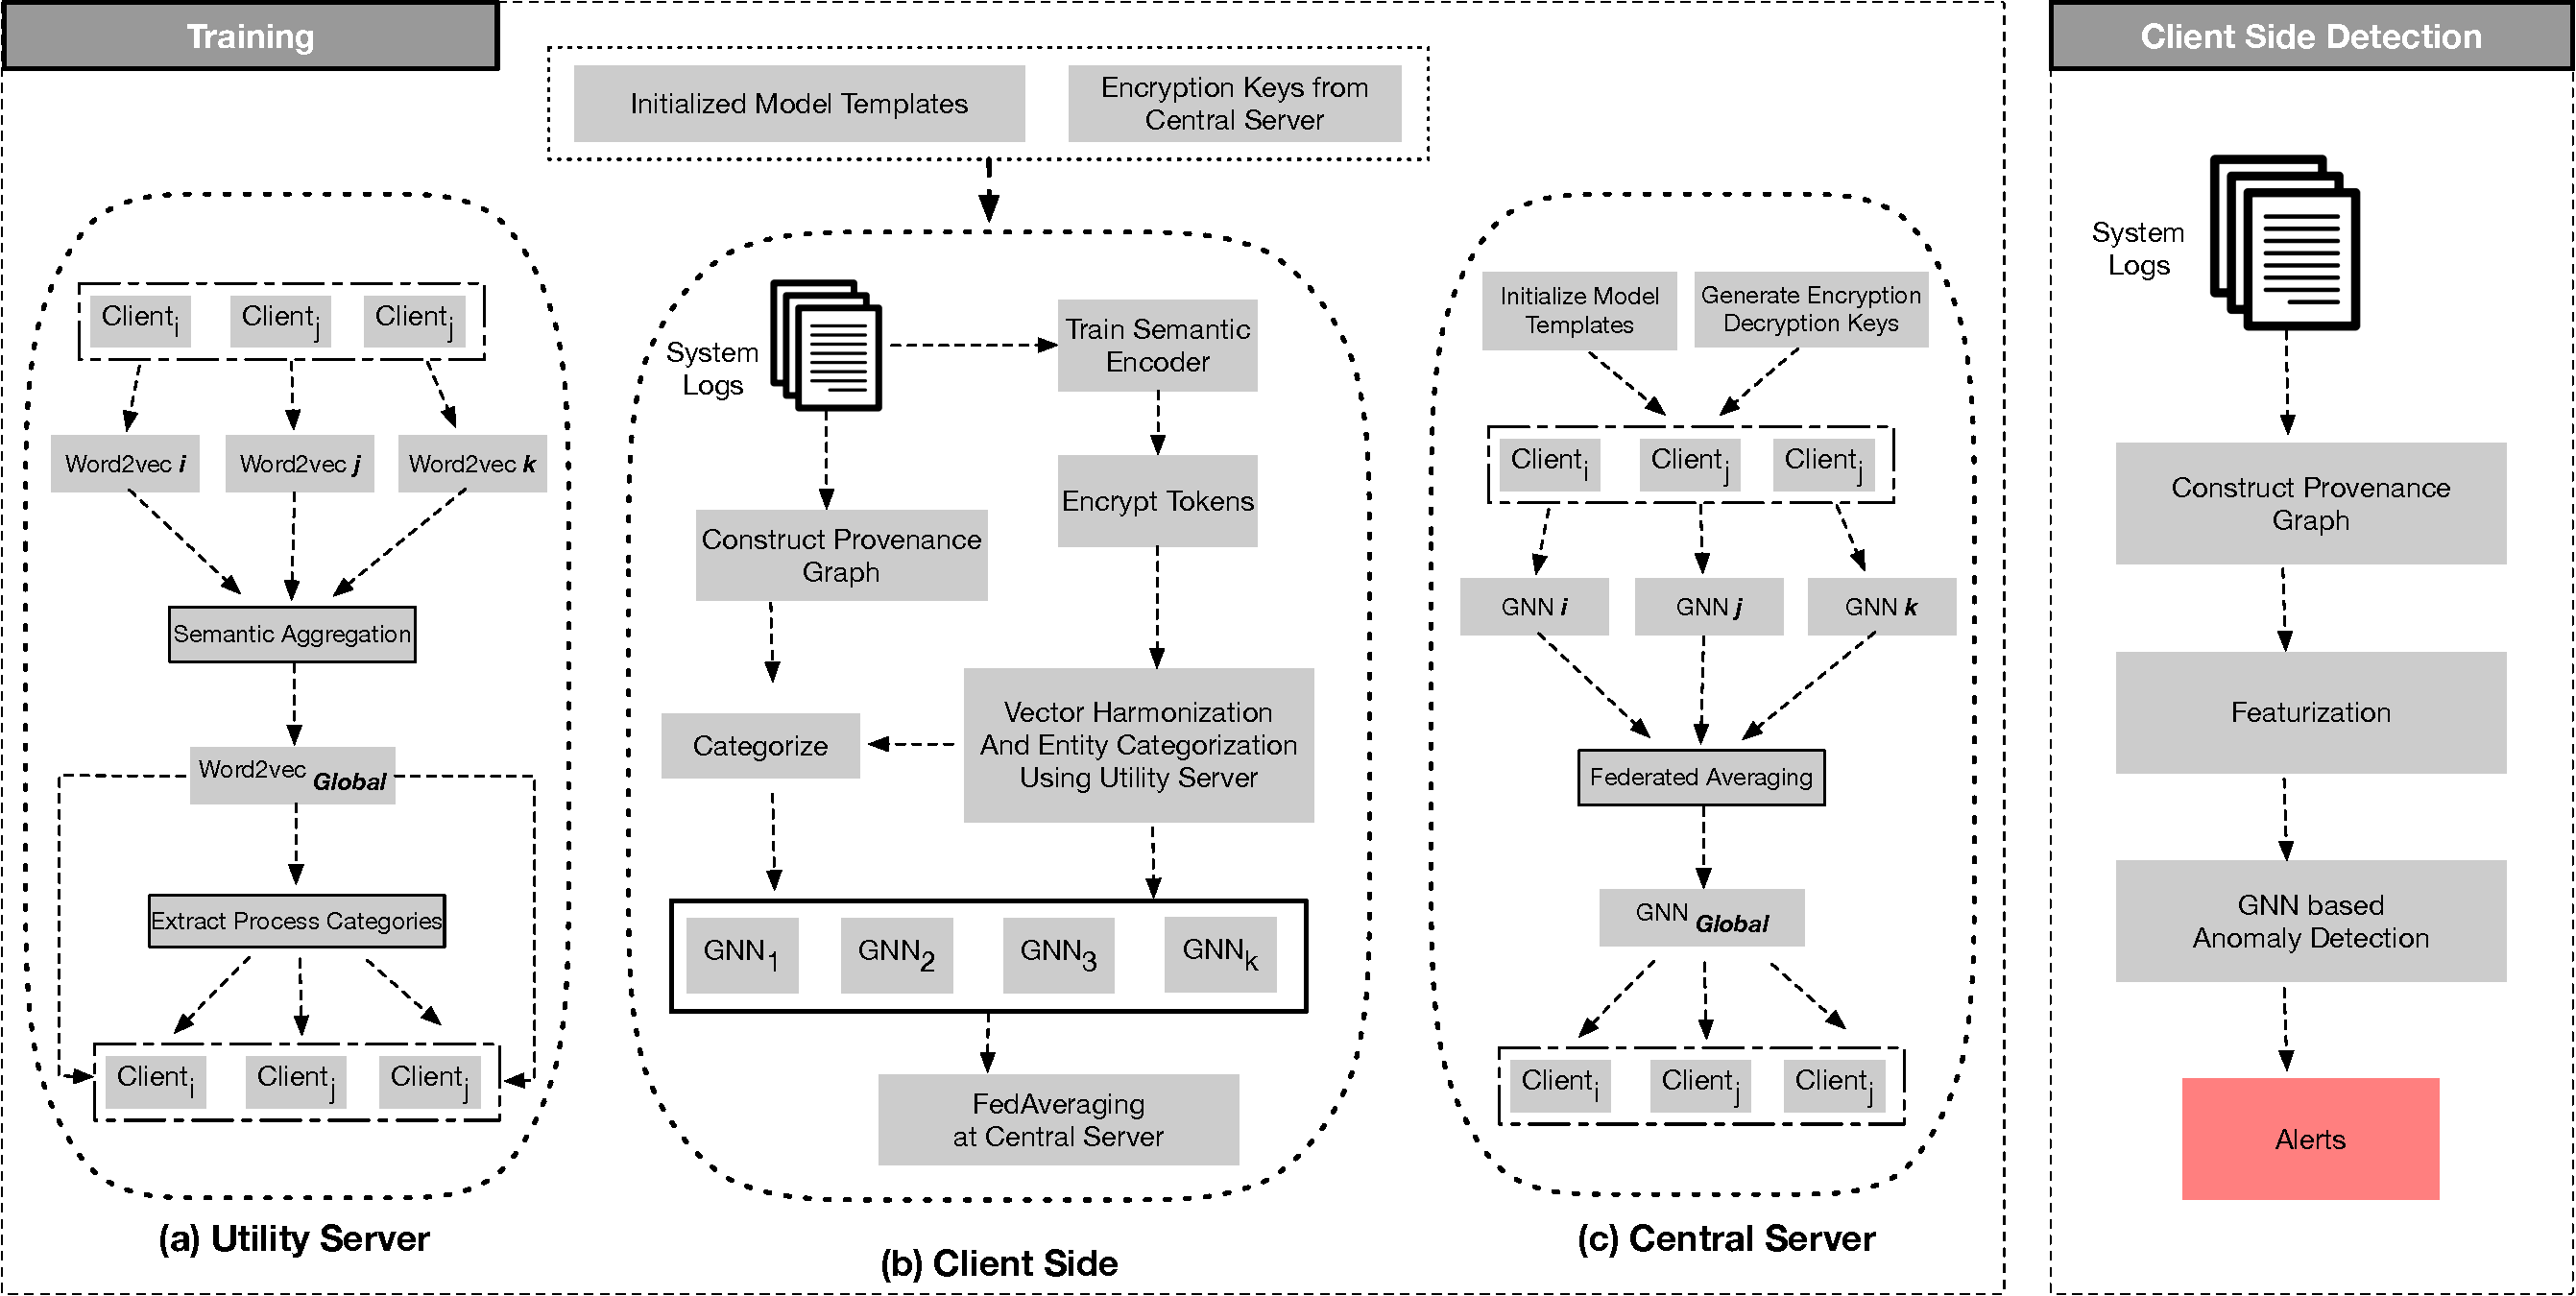
\includegraphics[width=0.90\textwidth]{fig/archv3.pdf}
  \caption{High-level architecture of \Sys. In the training phase, our system builds local provenance graphs for each client and trains an ensemble of \gnnshort models. Prior to this, we aggregate semantic models contextually for feature encoding. The local \gnnshort models participate in federated learning to develop a global \gnnshort model, which is then utilized for anomaly detection.}
  \vspace{-3ex}
  \label{fig:arch}
\end{figure*}

% \subsection{Overview}
\Sys comprises five key modules, starting with the \textit{Provenance Graph Constructor} module on each client machine, which transforms \logs into a provenance graph. While our approach to constructing provenance graphs builds on established methods~\cite{inam2023sok,nodoze2019,mpi+ma,loggc,lpm2015,hossain2017sleuth}, detailed information is provided in Appendix~\ref{sub:provconstruct}. The \textit{Semantic Featurization \& Harmonization} module (Section~\ref{semanfeat}) trains \wordvec models to encode semantic attributes and consolidates individual client models into a cohesive global model using a trusted utility server and encryption techniques. The \textit{Process Entity Categorization Module} (Section~\ref{sys:catg}) standardizes system entities across clients, ensuring uniformity in \gnnshort model training. The \textit{Federated Provenance Graph Learning Module} (Section~\ref{sys:fpgl}) then trains \gnnshort models on each client machine using harmonized semantic features, with the models aggregated on a central server through federated averaging. Finally, the \textit{Anomaly Detection Module} (Section~\ref{sys:anomaly_detection}) applies the unified global models for anomaly detection on each client machine. Figure \ref{fig:arch} illustrates the comprehensive architecture of \Sys, with further details in subsequent sections.


%\wajih{You need to talk about threat detection and alert generation.}

%\wajih{Give two or three sentences about the overall workflow. Think about what are the inputs, how the inputs are processed, and what are the outputs.} \wajih{Annotate "Audit Logs" in the Figure. Also use the word "Word2Vec" instead of Word2vec.}

%\wajih{Please divide this figure as we talked about. Use the color palette as I specified in the Dart Lab channel. Also, what is the difference between black and red edges? Could you add a legend for edges types?}

\subsection{Semantic Featurization \& Harmonization}
\label{semanfeat}

This module processes the provenance graph generated from \logs by transforming node attributes into feature vectors for the graph learning phase. Existing systems, such as Flash~\cite{flash2024} have demonstrated the effectiveness of utilizing semantic attributes of nodes to enhance detection performance. Building on this approach, we employ a \wordvec language model to encode these attributes into a vector format, \(\mathbf{v}\), where each attribute \(a\) is transformed into a vector \(v_a\). Each client independently trains a \wordvec model using their local \logs for feature encoding. Appendix~\ref{app:Word2vec:Semantic:Featurization} explains this process in detail.

However, before these models can be utilized to encode text attributes effectively, it is essential to contextually merge individual client \wordvec models into a unified model \( Word2vec_{Global} \) for use across all clients. This unification is crucial; without it, each client would produce a different encoding, \(v_a^i\), for identical inputs, where \(i\) denotes the client. The variability in feature vectors, \(\{v_a^1, v_a^2, \ldots, v_a^N\}\), for the same attribute \(a\) across \(N\) clients, would compromise the consistency of client-based \gnnshort models. To ensure uniformity, the feature vectors for overlapping attributes must be averaged across clients. Such averaging ensures consistency in the feature representation, enhancing the effectiveness of the downstream federated averaging technique by maintaining uniformity in the input space for the \gnnshort models across all clients.

The \wordvec model functions as a key-value store, with vocabulary tokens as keys, \(k\), and their corresponding vector representations as values, \(v_k\). To combine these models, we calculate the average vector of overlapping tokens from all client machines, creating a central model. The mathematical representation for averaging vectors of a token \(k\) across \(N\) clients is given by \(\bar{v}_k = \frac{1}{N}\sum_{i=1}^{N} v_{k,i}\) where \(\bar{v}_k\) is the averaged vector for token \(k\), and \(v_{k,i}\) is the vector representation of token \(k\) from the \(i\)-th client model.

However, transferring tokens -- containing sensitive data like process names, file names, and IP addresses -- to a central server could breach user privacy. To mitigate this, we employ a trusted utility server. Initially, the central server uses Fernet symmetric key encryption~\cite{ismail2020fernet,bokhari2016review} to generate an encryption key, which is distributed to clients. Clients then encrypt their \texttt{Word2vec} model tokens using the encryption key: \( E(v_{k}) = v_{k}^{'} \) and send them to the utility server. This server merges the encrypted models and dispatches the unified semantic vectors back to the respective clients, who decrypt them back: \( D(v_{k}^{'}) = v_{k} \).

This procedure ensures that neither the central server nor the utility server can access the actual token information, assuming no collusion between the two servers. The process is explained in detail in Algorithm~\ref{alg:secure_integration_averaging_word2vec}.

\begin{algorithm}[!t]
  \scriptsize
  \DontPrintSemicolon
  \SetKwInOut{Input}{Inputs}
  \SetKwInOut{Output}{Output}
  \Input{Client Word2Vec models $\{Word2vec_1, Word2vec_2, \ldots, Word2vec_k\}$.}
  \Output{Harmonized Word2Vec model $Word2vec_{Global}'$ sent to clients.}
  \BlankLine
  \tcc{Central server distribute symmetric encryption keys to each client.}
  \ForEach{client $C_i$}{

    Send $key$ to $C_i$\\
  }
  \tcc{Clients encrypt their model tokens.}
  \ForEach{client model $word2vec_i$}{
    $Word2vec_i \leftarrow$ EncryptModelTokens($Word2vec_i$, $E$) \tcc*{Encrypt tokens using $E$.}
    Send $Wor2vec_i$ to Utility Server\\
  }
  \tcc{Utility server merges encrypted models.}
  $TokenVectors \leftarrow$ InitializeEmptyDictionary()\\
  $TokenCounts \leftarrow$ InitializeEmptyDictionary()\\
  \ForEach{encrypted model $Word2vec_i$}{
    \ForEach{token $t$ in $Word2vec_i$}{
      $Vector \leftarrow Word2vec_i[t]$\\
      \eIf{$TokenVectors$.HasKey($t$)}{
        $TokenVectors[t] \leftarrow TokenVectors[t] + Vector$\\
        $TokenCounts[t] \leftarrow TokenCounts[t] + 1$\\
      }{
        $TokenVectors[t] \leftarrow Vector$\\
        $TokenCounts[t] \leftarrow 1$\\
      }
    }
  }
  \tcc{Average the vectors for overlapping tokens.}
  \ForEach{token $t$ in $TokenVectors$.Keys()}{
    $TokenVectors[t] \leftarrow TokenVectors[t] / TokenCounts[t]$\\
  }
  $Word2vec_{Global} \leftarrow$ NewModel($TokenVectors$, $EncryptedTokens$) \tcc*{Constructing a new harmonized model.}
  \ForEach{client $C_i$}{
    Send $Word2vec_{Global}$ to $C_i$\\
  }
  \BlankLine
  \Return{Harmonized model $Word2vec_{Global}$ has been dispatched to all clients.}\\
  \BlankLine
  \caption{Privacy preserving harmonization of \wordvec models.}
  \label{alg:secure_integration_averaging_word2vec}
\end{algorithm}

\subsection{Process Entity Categorization}
\label{sys:catg}

Our experimental results, presented in Table~\ref{categorized_gnn}, indicate that a single global \gnnshort model is not able to achieve good detection performance in an FL setting due to the diverse and heterogeneous distributions of clients' data. The disparity in data distributions among various clients leads to a significant challenge in effectively training a unified model that can generalize well across all clients. This diversity often results in poor model performance, as the global model struggles to capture the unique characteristics and patterns inherent in the data of individual clients.

To overcome this limitation, we developed a comprehensive framework that categorizes process entities across different clients into distinct groups. Our framework assigns process entities to specific categories, ensuring that each category is modeled by a dedicated submodel. This approach allows each submodel to better capture the unique distribution and intricate patterns of its assigned category, thereby improving the overall detection performance.

The framework operates by utilizing a central utility server, which plays a crucial role in the categorization process. Each client transmits a list of encrypted process names to the utility server to ensure privacy. The utility server then aggregates these lists and randomly splits them into \(k\) categories, where \(k\) is a predefined hyperparameter. We conducted experimentation to study the effect of \(k\) on detection accuracy, as detailed in Appendix~\ref{app:ablation}. Once the categorization is complete, the utility server sends these categorized lists back to the clients.

Upon receiving the categorized lists, clients organize their processes into \(k\) bins according to the assigned categories. This categorization ensures that each bin contains processes that are similar across different clients. Clients then use the processes in each bin to generate provenance subgraphs, which capture the interaction of these processes with other system objects. These subgraphs serve as the training data for an ensemble of \gnnshort models. Each submodel in the ensemble is trained on the subgraphs corresponding to its assigned category and participates in federated averaging.

This approach ensures a balanced and uniform segmentation of data across clients, maintaining consistency in the training datasets for each \gnnshort model before federated averaging. By dividing the overall task into sub-tasks (sub-models) and assigning them to different subsets of processes, the influence of clients with large datasets is diversified across multiple models. This prevents any single client from disproportionately influencing the outcome of the federated learning system. Each sub-model specializes in a different aspect of the data, capturing unique patterns and distributions. This specialization leads to more even contributions across the ensemble, enhancing the robustness and performance of the overall system.

\subsection{\fpgl}
\label{sys:fpgl}

% \wajih{In the arch figure, you have GNN Global notation, but you don't have it in the text below.}

The module performs graph representation learning in a federated manner. It includes a central server responsible for initializing the global \gnnshort models denoted by \(\{GNN_1, GNN_2, \ldots, GNN_k\} \) with random weights, which are then sent to all clients. These clients use their local process subgraphs and semantic feature vectors to train the \gnnshort models in an unsupervised way, following a training method similar to \flash. The \gnnshort model's objective is to classify each node entity into its corresponding type. The server then applies the federated averaging algorithm to merge the \gnnshort models into a set of global models (\( GNN_{Globals} \)). These models are then merged according to the process entity categories on which they were trained. This ensures that models with similar distributions are combined together to address the data heterogeneity problem. Specifically, for each submodel, the server aggregates parameters from \(N\) client models, to update the global model as follows:

\begin{equation}
\bar{w} = \frac{1}{N} \sum_{k=1}^{N}w_k
\end{equation}

where \(\bar{w}\) is the aggregated global model parameter, \(N\) is the number of client models and \(w_k\) is the parameter from the \(k\)-th client model.

The federated averaging process is repeated for a set number of rounds \(R\), and concludes when there is no further reduction in training loss. Algorithm~\ref{alg:federated_learning} shows the training and aggregation process of \gnnshort for a given process category and one round of FL.

% \begin{algorithm}[!t]
%   \scriptsize
%   \DontPrintSemicolon
%   \SetKwInOut{Input}{Inputs}
%   \SetKwInOut{Output}{Output}
%   \Input{Set of client models $\{GNN_1, GNN_2, \ldots, GNN_N\}$;\\}
%   \Output{Global GNN model $GNN_{Global}$.}
%   \BlankLine
%   \tcc{Initialize global GNN model with random weights for a given process Category.}
%   %\tcc{This initialization happens for the first FL round only.}
%   $G \leftarrow \text{InitializeRandomWeights}()$\\
%   \tcc{Distribute $GNN$ to all clients.}
%   \ForEach{client}{
%     Send $GNN$ to $Client_i$\\
%     $GNN \leftarrow \text{TrainOnLocalData}(ProcessCategory_i)$
%   }
%   \BlankLine
%   \tcc{Aggregate trained models from clients.}
%   $AggregatedWeights \leftarrow list([])$\\
%   \ForEach{client model $GNN_i$}{
%     $AggregatedWeights.append(\text{ExtractWeights}(GNN_i))$\\
%   }
%   \tcc{Apply federated averaging.}
%   $GNN_{Global} \leftarrow \text{FederatedAveraging}(AggregatedWeights)$\\
%   \BlankLine
%   \Return $GNN_{Global}$\\
%   \BlankLine
%   \caption{Federated Provenance Graph Learning}
%   \label{alg:federated_learning}
% \end{algorithm}

\subsection{GNN-based Anomaly Detection}
\label{sys:anomaly_detection}

\Sys employs a standard a node level detection methodology focusing on identifying irregular nodes through the comparison of their expected and observed types. This approach is grounded in a detailed analysis of both the surrounding structures and inherent properties of the nodes, to define normal pattern baselines for various node types. Typically, entities with malicious intentions display neighborhood structures and characteristics deviating from these established norms. In operational phases, the detection of anomalies that diverge from the pre-established node distribution patterns often results in their misclassification. The emergence of nodes misclassified in the system's output is indicative of potential security issues.

\Sys performs threat detection in a decentralized manner on client's provenance graphs (\( \{G_{c_1}, G_{c_2}, \ldots, G_{c_P}\} \)) in an organization. For a given provenance graph on a client machine containing nodes \(V\) and edges \(E\), \Sys uses the global \(\{GNN_1, GNN_2, \ldots, GNN_k\}\) \gnnshort models trained using federated learning. Each submodel performs inference on client's full provenance graph, utilizing the nodes' features \(X_v\) and the graph's adjacency matrix \(A\) to predict each node \(v\)'s label \(y_v^i\). A node \(v\) is identified as an anomaly if it is misclassified by all submodels, indicating that none of the submodels recognize the neighborhood structure or features displayed by this node. 

To regulate the frequency of alerts, we define a threshold \(T\) similar to \flash. This parameter sets a threshold on the likelihood of a classification being considered valid, with a higher value of \(T\) implying stronger confidence and increasing the probability of identifying anomalies. 